%===============================================================================
\subsubsection*{a)} \label{sec:3-1-a}
%===============================================================================

To implement the \code{DescretePDF} we modified \code{Mesh::activate} as seen in Listing \ref{lst:mesh-activate}. We first initialize \code{m\_distr} and the retrieve \code{triangleCount}. Since triangles are referenced via index, we can iterate each triangle area by using a simple \code{for}-loop. On each iteration we call \code{surfaceArea()} on each index. Its result is then appended to \code{m\_distr}. Finally, \code{m\_distr} is normalized.

\begin{lstlisting}[caption={\code{Mesh::activate}},label={lst:mesh-activate}]
void Mesh::activate() {
    m_distr.clear();
    uint32_t triangleCount{getTriangleCount()};
    for (uint32_t i = 0; i < triangleCount; ++i) {
        float area = surfaceArea(i);
        m_distr.append(area);
    }
    m_distr.normalize();
    
    ...
}
\end{lstlisting}

With \code{m\_distr} computed, implementing \code{Mesh::totalSurfaceArea} is trivial, as seen in Listing \ref{lst:mesh-total-surface-area}: We simply need to return the sum of \code{m\_distr}.

\begin{lstlisting}[caption={\code{Mesh::totalSurfaceArea}},label={lst:mesh-total-surface-area}]
float Mesh::totalSurfaceArea() const {
    return m_distr.getSum();
}
\end{lstlisting}

\code{Mesh::samplePosition} is a tad more complicated, as seen in Listing \ref{lst:mesh-sample-position}. First, since we need 2 random variables: One 1D variable for sampling \code{m\_distr}, and one 2D for sampling the \code{uv} on the triangle, we need to use \code{DiscretePDF::sampleReuse} instead of \code{DiscretePDF::sample}. It modifies \code{sample}, so we need to copy it first. Then we get the triangle vertices from the randomly chosen \code{index}; the code has been lifted from \code{Mesh::surfaceArea}. Then we sample a random \code{uv} using \code{Warp::squareToUniformTriangle}. Using that, we can now compute a point \code{p} on the triangle surface, using barycentric coordinates. Finally we compute the normal \code{n}, by taking the crossproduct of two of the triangle edges.

\begin{lstlisting}[caption={\code{Mesh::samplePosition}},label={lst:mesh-sample-position}]
void Mesh::samplePosition(const Point2f &sample, Point3f &p, Normal3f &n) const {
    // Copy the sample because sampleReuse modifies it
    auto reuse_sample = sample;
    
    // find triangle
    auto index = m_distr.sampleReuse(reuse_sample.x());
    auto i0 = m_F(0, index), i1 = m_F(1, index), i2 = m_F(2, index);
    const Point3f p0 = m_V.col(i0), p1 = m_V.col(i1), p2 = m_V.col(i2);
    
    // sample triangle point
    auto uv = Warp::squareToUniformTriangle(reuse_sample);
    
    // compute point
    auto u = uv.x();
    auto v = uv.y();
    p = (1.0f - u) * p0 + (u - v) * p1 + v * p2;
    
    // compute normal
    n = (p0 - p1).cross(p0 - p2);
    n.normalize();
}
\end{lstlisting}

%===============================================================================
\subsubsection*{b)}
%===============================================================================

\code{AreaLight::AreaLight}, \code{AreaLight::setParent}, \code{AreaLight::eval} are trivial to implement, as seen in Listing \ref{lst:trivial-area}. We add two private members \code{m\_Radiance} and \code{m\_Parent}, which are set in the constructor or its setter respectedly. \code{AreaLight::eval} just returns \code{m\_Radiance}.

\begin{lstlisting}[caption={Trivial area light implementations},label={lst:trivial-area}]
class AreaLight: public Emitter {
public:
    AreaLight(const PropertyList &propList) {
        m_Radiance = propList.getColor("radiance");
    }

    void setParent(NoriObject* obj) override {
        m_Parent = obj;
    }
    
    Color3f eval(Vector3f wi) const override {
        return m_Radiance;
    }
    
    ...
    
private:
    Color3f m_Radiance = {};
    NoriObject* m_Parent = nullptr;
};
\end{lstlisting}

\code{AreaLight::sampleDirect} and \code{AreaLight::pdfDirect} are a bit more involved. The implementation of \code{AreaLight::sampleDirect} is seen in Listing \ref{lst:area-sample-direct}. First, we assume \code{m\_Parent} to be a \code{Mesh}. We assert and then cast it to \code{Mesh}, so we can sample a Position on it, as implemented in Section \ref{sec:3-1-a}. We then populate \code{eRec}, similar to how \code{PointLight} does it. Finally, we compute the PDF. We return the radiance devided by the PDF, but only if the PDF is positive and not 0. Otherwise we return black.

\begin{lstlisting}[caption={\code{AreaLight::sampleDirect}},label={lst:area-sample-direct}]
Color3f sampleDirect(EmitterQueryRecord &eRec, Point2f sample) const override {
    // cast to mesh
    assert(m_Parent->getClassType() == m_Parent->EMesh);
    auto mesh = static_cast<Mesh *>(m_Parent);
    
    // sample position
    Point3f position;
    Normal3f normal;
    mesh->samplePosition(sample, position, normal);
    
    // fill eRec
    eRec.ep = position;
    eRec.measure = ESolidAngle;
    
    eRec.ws_wi = eRec.p - eRec.ep;
    eRec.distance = eRec.ws_wi.norm();
    eRec.ws_wi.normalize();
    
    Frame frame(normal);
    eRec.wi = frame.toLocal(eRec.ws_wi);
    
    auto pdf = pdfDirect(eRec);
    return pdf > 0.0f ? m_Radiance / pdf : Color3f{};
}
\end{lstlisting}

The formula for the PDF is

\[
p(\omega_i \mid \texttt{p}) = \frac{1}{A} \cdot \frac{dA}{d\omega_i} = \frac{1}{A} \cdot \frac{r^2}{\cos\theta_e}
\]

It's implementation is seen in Listing \ref{lst:area-pdf-direct}. We assert and cast to \code{Mesh} again. $A$ is the the total surface area of the mesh, which we retrive by calling \code{mesh->totalSurfaceArea()}. $r$ is the distance between sampled point and emitter, which is already stored in \code{eRec.distance}. To compute $\cos\theta_e$, we use a little trick. The dot product is defined as:

\[
a \cdot b = \|a\| \, \|b\| \cos\theta
\]

When $a$ and $b$ are normalized, it simplifies to:

\[
    a\cdot b = \cos\theta
\]

Now, $a=\omega_i$ and $b$ is the surface normal. But in the local shading frame, the surface normal is $(0, 0, 1)$. Therefore:

\[
    \cos\theta = a\cdot b = \omega_i\cdot (0, 0, 1) = \omega_{i.1} \cdot 0 + \omega_{i.2} \cdot 0 + \omega_{i.3} \cdot 1 = \omega_{i.3}
\]

$\omega_{i.3}$ is simply the $x$-coordinate of $\omega_i$, which we retrive by calling \code{eRec.wi.z()}. Finally we compute the PDF by throwing the gathered values together. If $\cos\theta_e$ is negative, we return 0.

\begin{lstlisting}[caption={\code{AreaLight::pdfDirect}},label={lst:area-pdf-direct}]
float pdfDirect(const EmitterQueryRecord &eRec) const override {
    // cast to mesh
    assert(m_Parent->getClassType() == m_Parent->EMesh);
    auto mesh = static_cast<Mesh *>(m_Parent);
    
    // compute pdf
    auto A = mesh->totalSurfaceArea();
    auto r = eRec.distance;
    auto cos_theta = eRec.wi.z();
    auto pdf = r * r / (A * cos_theta);
    
    return cos_theta > 0.0f ? pdf : 0.0;
}
\end{lstlisting}

%===============================================================================
\subsubsection*{c)}
%===============================================================================

In \code{DirectLightIntegrator}, nothing had to be changed. We simply used the sample solution, which worked fine out of the box. We assume the code, which the exercise arsks for, is listed in Listing \ref{lst:area-direct-light-integrator}. When the intersection \code{its} is an emitter, it's evaluated added to the returned radiance.

\begin{lstlisting}[caption={\code{DirectLightIntegrator}},label={lst:area-direct-light-integrator}]
class DirectLightIntegrator : public Integrator {
public:
    ...
    
    Color3f Li(const Scene *scene, Sampler *sampler, const Ray3f &ray) const {
        ...

        const Emitter* emitter = its.mesh->getEmitter();
        if (emitter)
            Li += emitter->eval(its.toLocal(-ray.d));

        return Li;
    }
    
    ...
};
\end{lstlisting}

%===============================================================================
\subsubsection*{d)}
%===============================================================================

\begin{figure}[htbp]
    \centering
    \begin{subfigure}{0.32\textwidth}
        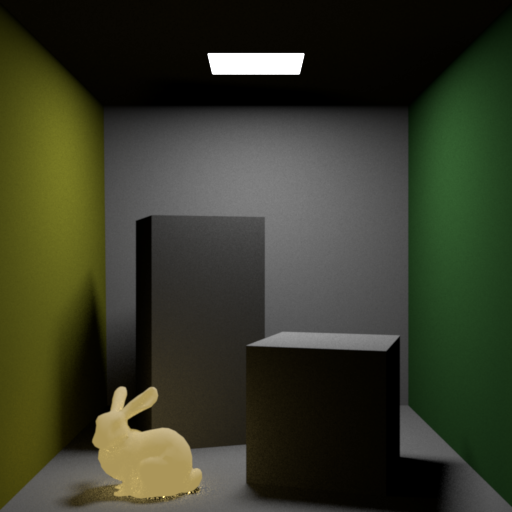
\includegraphics[width=\linewidth]{pictures/cbox-direct-512spp-ref.png}
    \end{subfigure}
    \hfill
    \begin{subfigure}{0.32\textwidth}
        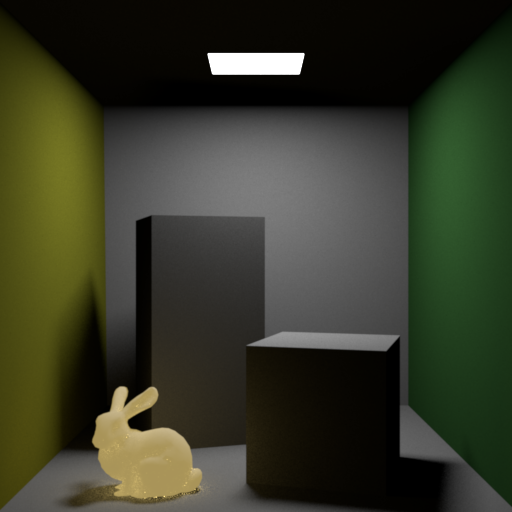
\includegraphics[width=\linewidth]{pictures/cbox-direct.png}
    \end{subfigure}
    \hfill
    \begin{subfigure}{0.32\textwidth}
        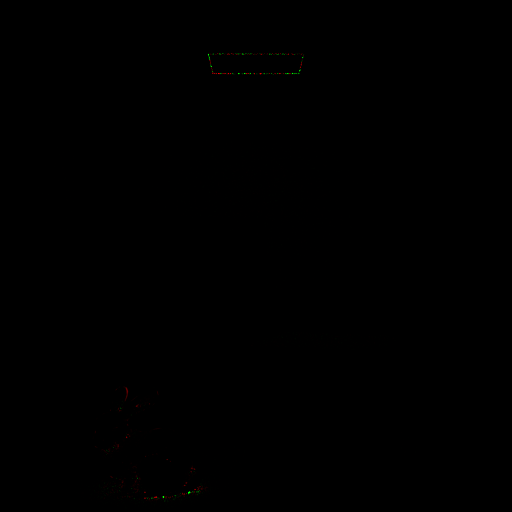
\includegraphics[width=\linewidth]{pictures/compare_3_1.png}
    \end{subfigure}
    \caption{The reference image (left) and our result (center) compared (right). Our result was rendered using 1024 samples. The pictures are pretty much identical. The only differences are in the edges of the emitters, which we think are artifacts due to different sample counts or nori versions.}
    \label{fig:comparison-3-1}
\end{figure}